% This is the aspauthor.tex LaTeX file
% Copyright 2010, Astronomical Society of the Pacific Conference Series

\documentclass[11pt,twoside]{article}
\usepackage{asp2010}

\resetcounters

\bibliographystyle{asp2010}

\markboth{Feng and Brunner}{Probabilistic Galaxy Classification}

\begin{document}

\title{New Probabilistic Galaxy Classification in Large Photometric Surveys}
\author{Feng Liang$^1$ and Robert J. Brunner$^2$
\affil{$^1$Department of Statistics, University of Illinois}
\affil{$^2$Department of Astronomy, University of Illinois}}

\begin{abstract}
A number of different projects have or soon will map the sky in part to better constrain the cosmological parameters driving the evolution of our Universe. One of the most important and least quantified steps in this process is the task of efficiently identifying galaxies within these large data sets. Generally, simple parameter cuts have been used, for example the SDSS cut on the difference between a PSF and model magnitude in the r-band. While this approach can be efficiently implemented and is easy to understand, it has been shown to be ineffective at brighter magnitudes than originally suspected. Thus, we are applying powerful statistical techniques such as support vector machine and non-parametric bayesian clustering to this challenge with the goal of developing a probabilistic galaxy classification that can be reliably extended to fainter magnitudes, thereby increasing the precision of future cosmological measurements.
\end{abstract}

\section{Introduction}

While our goal is to develop new star/galaxy classification techniques for the data now coming from the Dark Energy Survey (DES) and forthcoming Large Synoptic Survey Telescope (LSST), our current efforts use the data from the seventh data release from the Sloan Digital Sky Survey~\citep{york00}. Our full sample includes all objects from the SDSS photometric catalog with either a $g$, $r,$ or $i$ band detection brighter than 23rd magnitude. The SDSS developed a classification system that uses a concentration index~\citep{scranton02}, which quantifies the degree to which an object�s flux is spread out in an image. Stars are point sources, so they tend to be fairly concentrated, while galaxies are more extended. This concentration parameter is defined as the difference between the point spread function (PSF) magnitude and the model magnitude. The former measures the light from a source in a fixed size aperture (\textit{e.g.}, circle), while the latter fits a model to the light profile and measures the light form a source in a dynamically sized aperture. 

In the left panel of Figure~\ref{sdsssg}, we present the normalized, two-dimensional histogram of the distribution of $r$-band PSF magnitude versus the $r$-band concentration index for sources in the SDSS that were obtained in good observing conditions (the quality of observations can strongly affects the concentration measure). In this image, the official SDSS classification of 0.145 is shown in the magenta dashed line. To the left of this line is the stellar distribution, which is quite concentrated at bright magnitudes (smaller values of the PSF magnitude). To the right are the galaxies, which are more spread out since galaxies are more extended. 

\articlefiguretwo{good-data-class.eps}{good-data-slice.eps}{sdsssgo}{\textit{Left:} The concentration-magnitude diagram showing the official SDSS classification line in magenta, with sources to the left being classified as stars, while sources to the right are  classified as galaxies. \textit{Right:} The concentration density plots for objects with $r \in [19.5, 20.0]$ and $r \in [21.0, 21.5]$, showing how the different mixtures vary with magnitude.\label{sdsssg}}

%\begin{figure}
%\begin{center}
%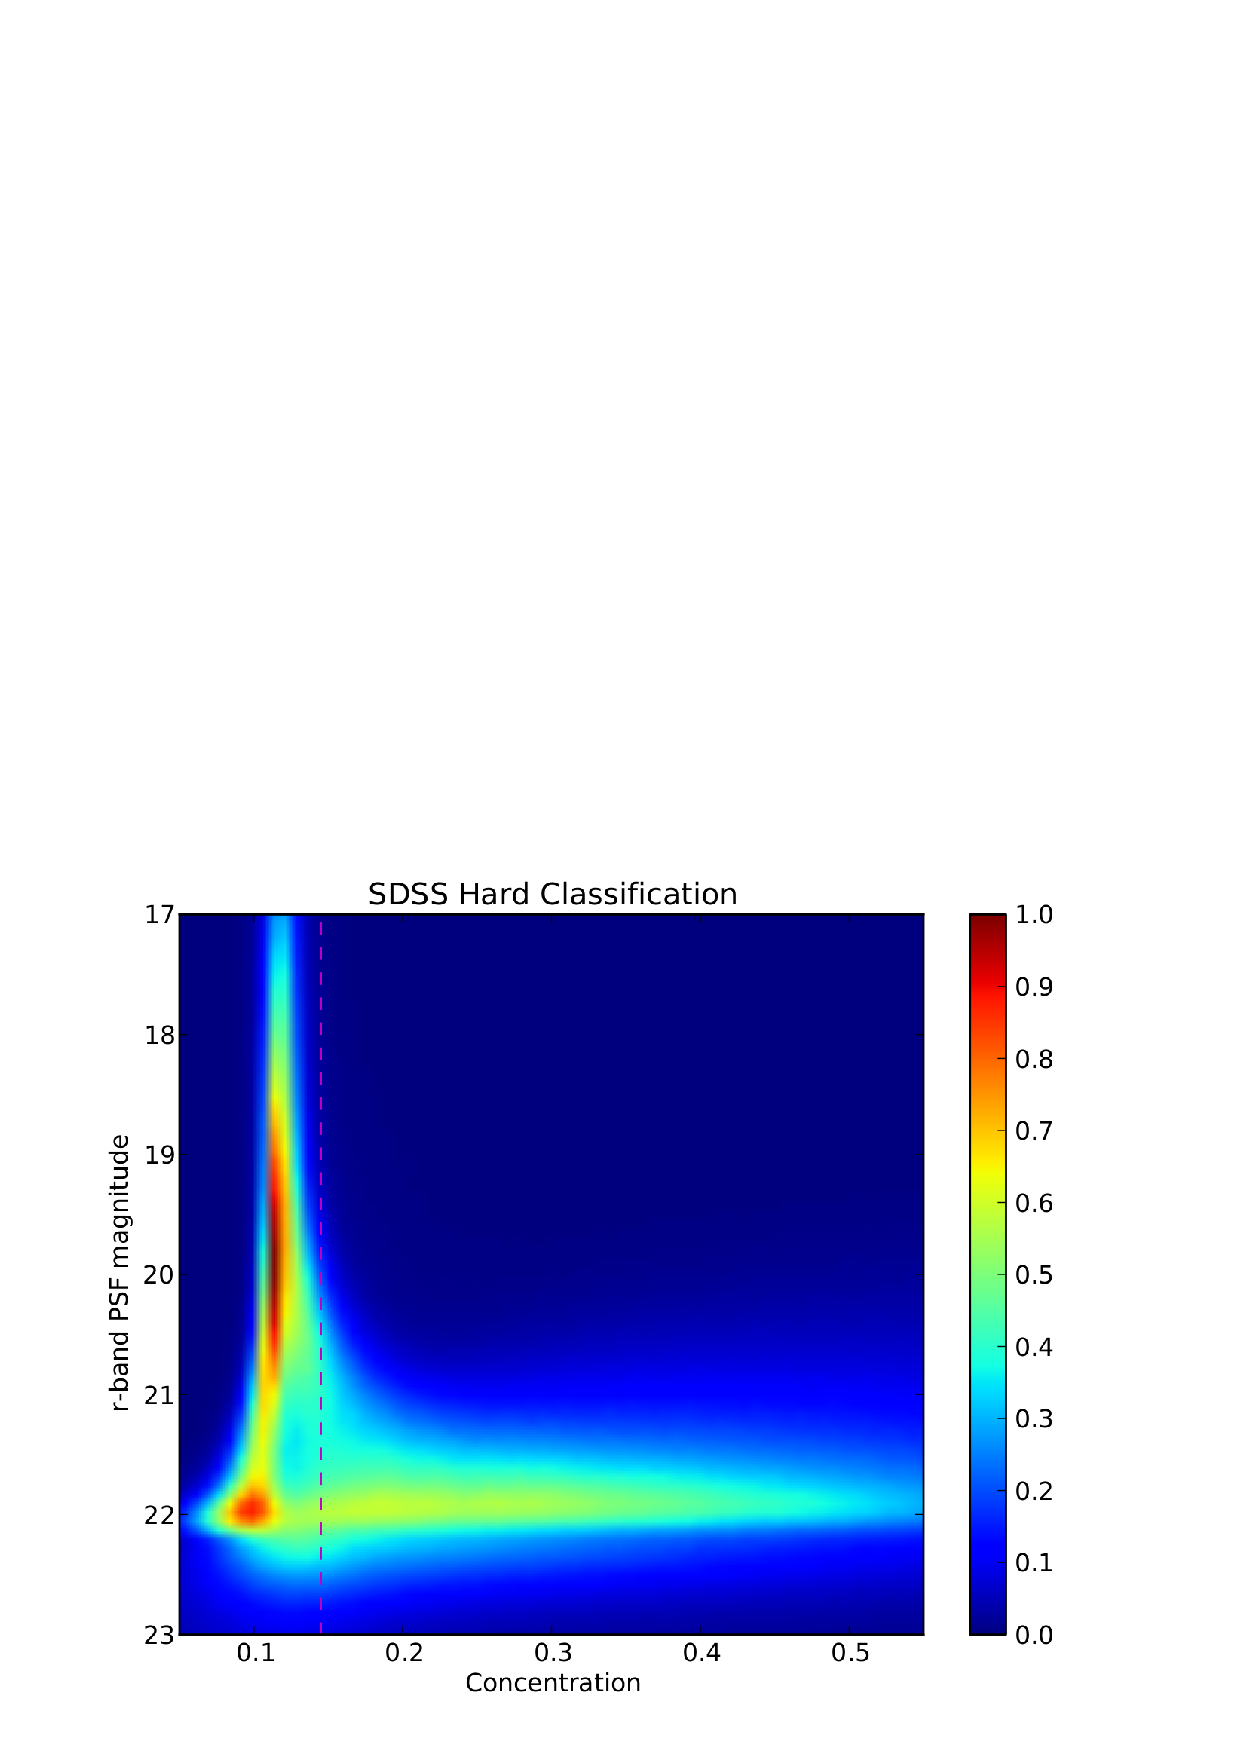
\includegraphics[width=3.5in]{good-data-class.pdf}
%\end{center}
%\caption{Concentration-magnitude diagram for regions of good observing conditions. The dashed line is the official SDSS classification line, where the left is classified as stars and the right is classified as galaxies.}
%\end{figure}

At fainter magnitudes, where the light measures are lower signal-to-noise, the two distributions begin to merge, complicating the classification. This is more clearly shown in the right panel of Figure~\ref{sdsssg}, where we have taken a slice through the two-dimensional histogram shown in the left panel of  Figure~\ref{sdsssg}, and plotted the distribution of all sources in two PSF magnitude ranges against concentration index. For the brighter sources, there are clearly two distributions. However, at fainter magnitudes, the two distributions are less cleanly separated and even show mixing beyond what might be expected simply from being lower signal-to-noise data. This reinforces the need for a more robust, probabilistic classification approach.

%\begin{figure}
%\begin{center}
%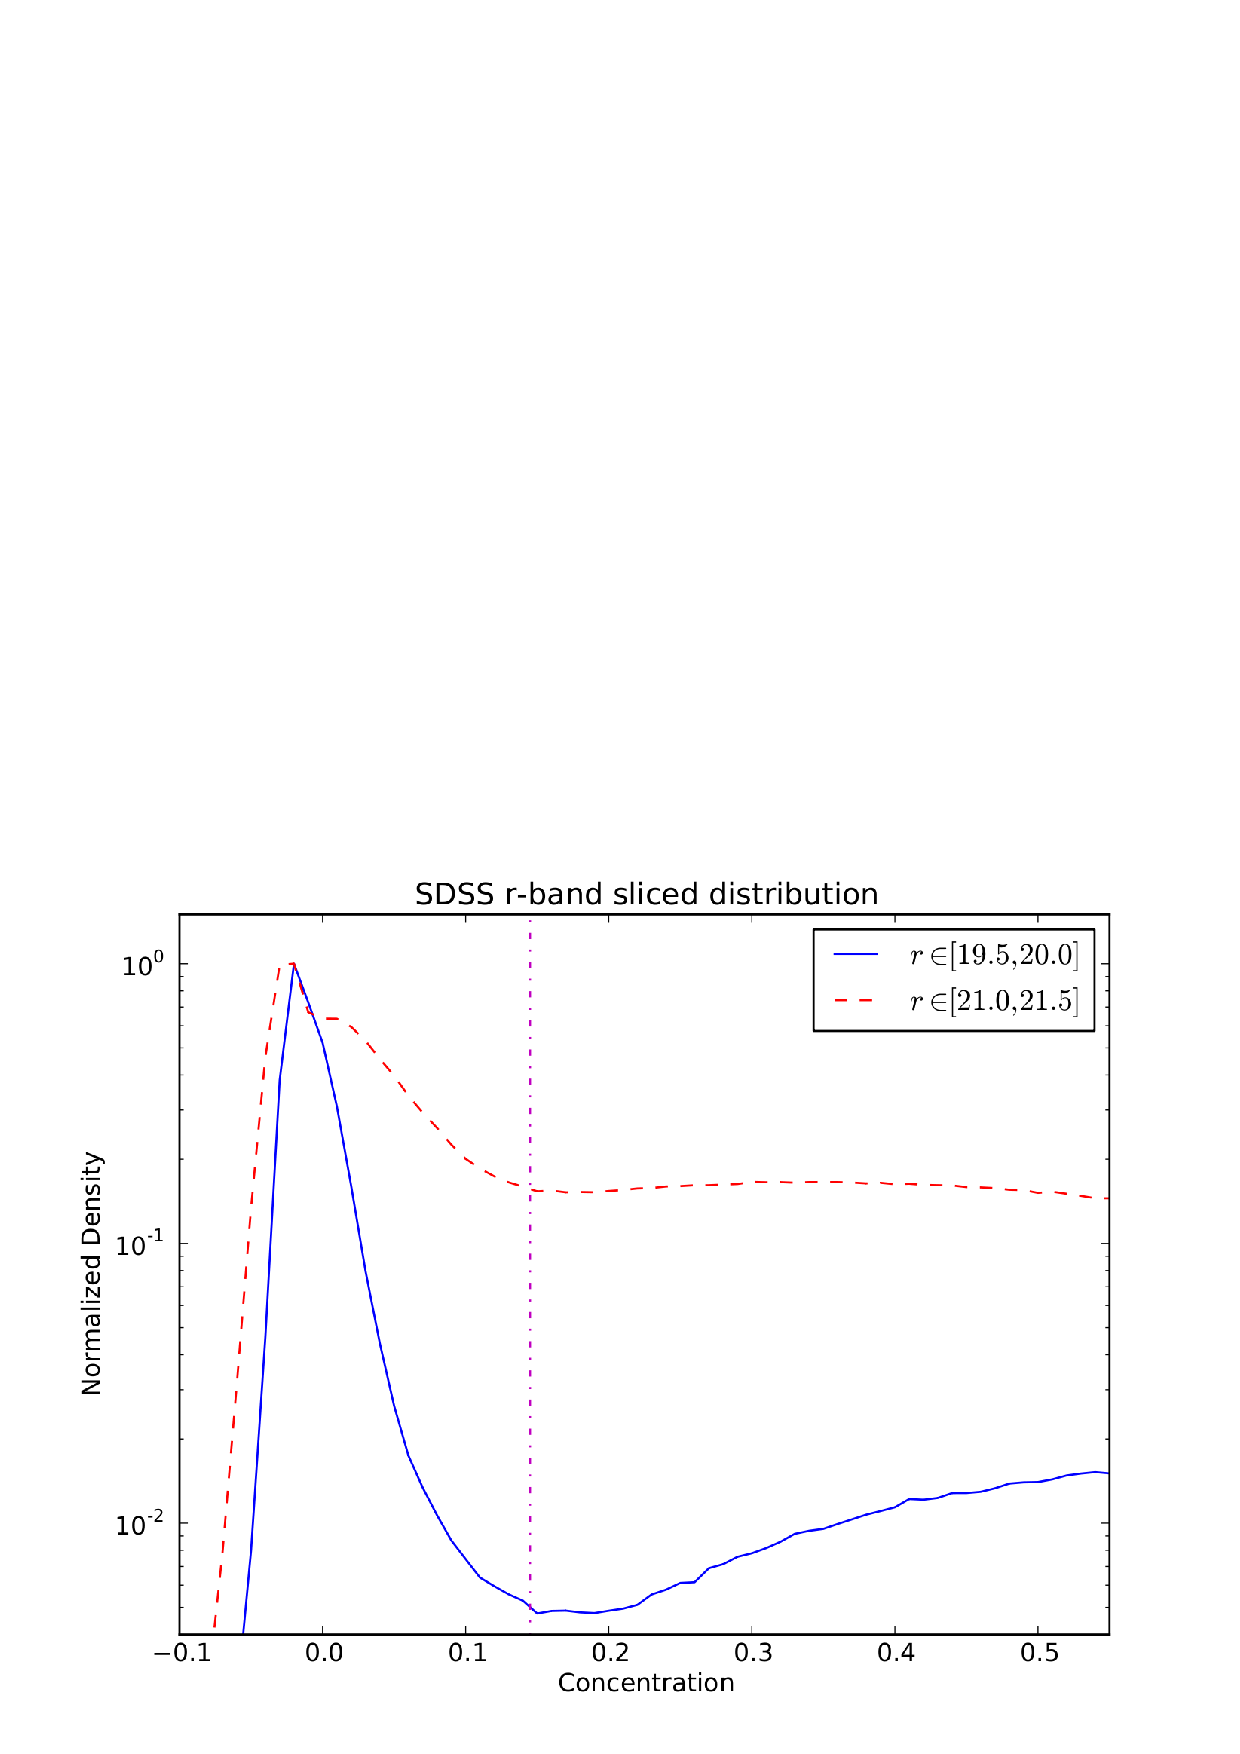
\includegraphics[width=3.5in]{good-data-slice.pdf}
%\end{center}
%\caption{Concentration density plots for objects with $r \in [19.5, 20.0]$ and $r \in [21.0, 21.5]$.}
%\end{figure}

%\section{Data}
%briefly describe SDSS data. Its location. why SDSS? What does SDSS use? Stripe 82 truth data for classification

%For figure, could show something about S/G being a problem in SDSS, or something from the work I have done with an undergrad on fitting a mixture model to the SDSS technique.

\section{A New Probabilistic Classification}

By applying Bayes formula, we have
\[ P(G \mid X) = \frac{P(X \mid G) P(G\mid I)}{P(X \mid I)}
\]
for the the probability that a source is a galaxy conditioning on its multi-dimensional photometric attributes $X \in \mathbb{R}^p$.  $\pi(G \mid I)$ and $P(X \mid G)$ represent the prior distribution and the likelihood of $X$ when the source is a galaxy, respectively. We can write a similar relationship for the probability that a source is a star (S), or any other object of interest (\textit{e.g.}, artifact, meteorite, satellite, AGN, \textit{etc.}), while the denominator is simply a normalization constant. %The data $X$ 

But we are now left with the question, how do we estimate the distribution for each class: $P(X \mid G)$ and $P(X \mid S)$? There are no theoretical templates when $X$ represents the measured photometric attributes of interest, which may contain many heterogenous attributes. If we have a large amount of training data that has been correctly classified, we could divide the data into two categories: stars and galaxies, and estimate the two distributions~\citep[\textit{e.g.},][]{fadely12}. For most survey data, however, we only have labels returned by the reduction software (\textit{e.g.}, the SDSS hard-cut classification); and, as we have demonstrated, those labels are not always reliable. Of course, for some parts of the sky we can obtain a set of reliable classification labels, \textit{e.g.}, if deeper photometric data or spectroscopic classifications are available. Thus, in a formal sense, star/galaxy classification  is essentially a semi-supervised learning problem, where some data  are labeled and some are not (\textit{i.e.}, some labels are not reliable, and should not be used). 

We now provide an outline of our new approach, which has two components:  (1) Model $X$ by a mixture 
\[ P(X) = \sum_{k=1}^K w_k P_k (X \mid \theta_k), \]
where $w_k$ is the prior probability of an object belonging to the $k^{th}$ cluster and $\theta_k$ are the different photometric attributes. (2) For a new object with photometric attributes $X^*$, we define a classification probability as
\[ P(G \mid X^*) = \frac{\sum_{k=1}^K \pi_k w_k P_k (X^* \mid \theta_k)}{\sum_{k=1}^K w_k P_k( X^* \mid \theta_k)}, \]
where $\pi_k$ is the probability of sources in the $k^{th}$ cluster being a galaxy, the numerator is an average of the $\pi_k$'s weighted by the cluster-specific likelihood, and the denominator is just a normalizing constant. The probability $\pi_k$ can be either supplied by experts or calculated by the empirical frequency of galaxies in the $k^{th}$ cluster. 

\section{Nonparametric Bayesian Clustering}

We introduce the latent cluster indicator variables $Z_1, \dots, Z_n$, which take values from $1$ to $K$ so that $X_i \mid Z_i = k  \sim P_k( \cdot \mid \theta_k).$ But we now have another issue, what value do we use for $K$? A natural, first choice would be to assume $K=2$: one cluster for stars and one cluster for galaxies; however, stars and galaxies have sub-types, and their distributions within each cluster are known to be heterogeneous. Instead, we model $Z_1, \dots, Z_n$ by a Chinese Restaurant Process (CRP), in which we do not need to specify $K$. Instead we treat $K$ as an unknown parameter. In particular, a CPR models $Z_i$'s sequentially as follows: $Z_1 =  \mathbf{1}(Z_1 = 1)$ and for $n > 1$,
\[
Z_{n} \mid Z_1, \dots, Z_{n-1} \sim  \sum_{i=1}^{n-1} \frac{1}{n-1 + \alpha} \mathbf{1}(Z_n = Z_i) + \frac{\alpha}{n-1+ \alpha} \mathbf{1}(Z_n = m+1), 
\]
where $m$ at the last step denotes the number of clusters formed by the previous $(n-1)$ samples. For an alternative description, the $1^{st}$ customer entering a Chinese restaurant sits at Table 1. When the $2^{nd}$ customer enters: she can either sit with the $1^{st}$ customer at Table 1 with probability $1/(1 + \alpha)$, or sit at a new table (\textit{i.e.}, Table 2)  with probability $\alpha / ( 1 + \alpha)$. This process continues, until finally, for the last customer, she can either start a new table (\textit{i.e.}, Table $m+1$) or sit at any of the $m$ existing tables. It is easy to see that the CRP naturally forms clusters among the $n$ samples. And most importantly, the number of clusters is not pre-fixed \textit{a priori}, but treated as a random variable. 

\section{Utilizing the Label Information}

Clustering models based on CRP are known as Dirichlet Process Mixture (DPM; ~\citealt{antoniak74}) models, and have been used previously in other applications. However, we still have a gap between DPM and the problem of galaxy classification, how do we encourage stars to cluster with stars and galaxies to cluster with galaxies? We can discourage the mixing of stars and galaxies in a cluster by specifying  constraints. Without a loss of generality, assume we have the true labels (\textit{i.e.}, star or galaxy) for the first $m<n$ objects. We can construct an $m$-by-$m$ symmetric matrix $E$, where $E(i,j) = 1$ if object $i$ and object $j$ are both stars (or galaxies), and $-1$ if they are different. That is,  $E$ represents the collection of all the pairwise constraints. We treat them as ``soft" constraints and model $E_{ij}$ (where $i<j$) as
\[
\left \{ \begin{array}{ll} P(E_{ij} = 1 \mid Z_i = Z_j) = p, & P(E_{ij} = -1 \mid Z_i = Z_j) = 1- p, \\
P(E_{ij} = -1 \mid Z_i  \ne Z_j) = q, & P(E_{ij} = 1 \mid Z_i \ne  Z_j) = 1-q.
\end{array} \right.
\]
Here $p$ and $q$ represent the chance of agreement between the true labels and the clustering indicators, which can be learned from the data adaptively. We can see the role these constraints play by looking at how the distribution of $Z_i$'s is affected by $E$:
$$
P(Z_i = k) \mid \mathbf{Z_{[-i]}}, E)  \propto  P(Z_i \mid Z_{[-i]}) 
  \times P(E_{i1}, \dots, E_{in}).
$$
The $1^{st}$ term, $P(Z_i \mid Z_{[-i]})$, is from the CRP, which is the same as the CRP sampling with $Z_i$ being the last customer entering the restaurant (due to the  exchangeability of CRP). The 2nd term, $P(E_{i1}, \dots, E_{in})$, specified before, depends on the proportion of stars and galaxies on the $k^{th}$ table. So when the $i^{th}$ customer picks her table, she not only favors large tables, but also tables with a high-percentage of stars. 
 
\section{Computation: Variational Methods}

To finish up the Bayesian hierarchical model, we can add priors on other parameters, such as Beta priors for $p$ and $q$, and priors for $\theta_k$'s. The last step is to compute the posterior distribution of the unknown parameters given the data. It is not difficult to derive a Gibbs sampler to do the posterior sampling. However, Gibbs samplers or any other variants of MCMC do not scale well to very large data. Instead we will derive an approximation algorithm based on variational methods~\citep{bishop06}. The idea is to cast the problem of estimating the posterior distribution as an optimization problem, where we try to minimize the Kullback-Leibler distance between the true posterior distribution $P( \Theta \mid X_{1:n})$ and our approximation $Q(\Theta)$, 
\[ J (Q) = \int Q(\Theta) \log \frac{P(\Theta \mid X_{1:n}) P(X_{1:n})}{Q(\Theta)} d \Theta. \]
If we divide the parameter into blocks, $(\Theta_1, \dots, \Theta_l)$, and approximate the posterior by $ Q(\Theta) = Q_1(\Theta_1) \times  \dots \times Q_l(\Theta_l)$; we can apply a coordinate-decent algorithm to sequentially solve $Q_1, \dots, Q_l$.

%\acknowledgements

%Any thanks to funding agencies.

\bibliography{../../editor}


\end{document}
